% !TEX encoding = UTF-8 Unicode
%!TEX root = memoria.tex
% !TEX spellcheck = es-ES
%%=========================================
\chapter{Desarrollo}
%%=========================================
\section{Estructura del experimento}
\subsection{Estructura de directorios}
\subsection{Configuración del experimento}
%%=========================================
\section{Módulo preprocesado}
\subsection{Parametrización}
\subsection{Salidas}
%%=========================================
\section{Módulo extracción de mapa cerebral}

CanICa eun un método ICA para el análisis de datos fMRI a nivel de grupo. Comparado con otras estrategias, aporta un modelo de grupo bien controlado, así como un algoritmo umbral que controla la especificidad y sensibilidad con un modelo explicito de la señal \cite{canica}


\subsection{Parametrización}
\subsection{Salidas}
%%=========================================
\section{Módulo extracción de regiones}
\subsection{Parametrización}
\subsection{Salidas}
%%=========================================
\section{Módulo para el cálculo de entropía}

\subsection{Densidad Espectral de Potencia}

El módulo \href{http://nipy.org/nitime/api/generated/nitime.algorithms.spectral.html}{algorithms.spectral} premite estimar la representación de las imágenes en el dominio de la frecuencia. Este módulo permite la utilización de varios métodos en el mismo API común.

%\begin{figure}[H]
%  		\centering
%    	\includegraphics[scale=0.5]{img/psd/filtering_fmri_01.png}
%  		\caption{Espectro de potencia para los diferentes médotodos del API}         \label{desa:psd1}
%\end{figure}

Para obtener la PSD se utiliza utiliza el método de Welch a fin de determinar las características de potencia de la señal previamente procesada.Los valores que se obtienen son finitos y están divididos por el periodo de la señal. Con la PSD podemos conocer la dispersión de la señal en términos de potencia, por lo que serían parámetros de interés que permiten el aprendizaje de algoritmos de clasificación, además del cálculo de las técnicas no-lineales de análisis como es la SSE.

\subsection{Entropía Espectral de Shannon}

La función que permite el cálculo de la SSE se basa en el siguiente algoritmo:

\begin{enumerate}
	\item Se obtiene el espectro de la señal $X(t)$
	\item Se normaliza el PSD a fin de que pueda ser interpretado como una función de densidad
	\item Finalmente se calcula la SSE usando la formula estandar para la entropía: 
	$$SSE=-\sum_{i=f1}^{f2}p_{i}\ln{p_{i}}$$
\end{enumerate}

Donde $f1$ y $f2$ son las frecuencias de corte.

La SSE permite cuantificar la distribución de potencia del espectro de una señal. Un valor de
SSE elevado indica que el espectro de la señal es uniforme y tiene una distribución en
frecuencia bastante amplia, mientras que un valor bajo se corresponde con un espectro
donde la potencia se encuentra condensada en un rango de frecuencias menor. Además, si
se compara varias señales entre sí, un valor menor de Entropía Espectral sugiere que esa
señal es más regular y predecible.

\subsection{Entropía de permutación}

En el capítulo 3 se explica el concepto de entropía de permutación, para clarificar este concepto se expone un ejemplo numérico de construcción de los patrones. Para una dimensión embebida $D=3$ el vector correspondiente con el instante $s=1$ es $(3,1,4)$, el vector es ordenado de forma ascente, obteniendo $(1,3,4)$, y el correspondiente patrón de permutación $\pi=(102)$. Para $s=2$, el vector con los valores es $(1,4,1)$, obteniendo la permutación $\pi=(021)$. Tener en cuenta que si dos valores son iguales serán asignados en orden temporal de aparición.

Para implementar la PE dada una serie temporal $\{x_{i}\}$ de longitud N se ha seguido el algoritmo:
\begin{enumerate}
	\item Se define el orden de la permutación \textit{n}. Esto provee de la capacidad de establecer patrones $\pi_{j}=(j=1,\dots,n!)$ que se generará a partir de los números $1,\dots, n.$ como se puede ver en la figura \ref{desa:pe1}.
	
	\begin{figure}[H]
  		\centering
    	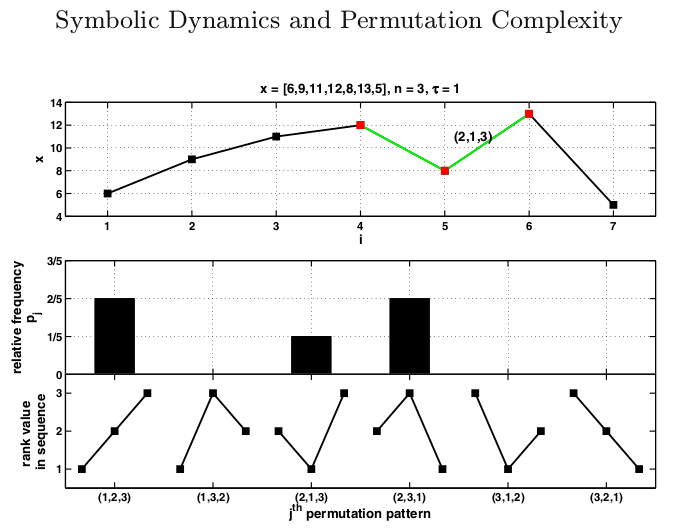
\includegraphics[scale=0.5]{img/pe_graph.png}
  		\caption{Ejemplo del cálculo de la entropía de permutación}\label{desa:pe1}
	\end{figure}
	\item Se crean las permutaciones dado el orden
	\item Inicializar $i=1$ como el índice de la serie de tiempo considerada $\{X_{i}\}_{i=1,\dots,N}$ y el contador $z_{j}=0$ para cada $\pi_{j}$
	\item Calcular el ranking de los valores en la secuencia $x_{i},\dots,x_{i+D-1}$ como $r_{i},\dots,r_{i+D-1}$: Los indices de los valores en orden ascendente.
	\item Comparar el ranking obtenido el paso anterior con todos los patrones de la permutación e incrementar el contador de patrones iguales $\pi_{j}=r_{i},\dots,r_{i+n-1}$ en uno $z_{j}=z_{j}+0$
	\item En caso de que $i \leq N-n-1$ entonces se incrementará i en uno $i=i+1$ y comenzamos por el calculo del ranking de nuevo. En otro caso continuar con el siguiente paso.
	\item Calcular la frecuencia relativa de todas las permutaciones $\pi_{j}$ siguiendo la ecuación:
		$$p'_{j}=\frac{z_{j}}{\sum{z_{k}}}$$ y estimar su probabilidad $p_j$
	\item Realizar el cálculo de la entropía dada la ecuación \ref{ecuaciones:3}
\end{enumerate}

\subsubsection{Selección de parámetros}
\cite{pe2}
\subsection{Parametrización}
\subsection{Salidas}
%%=========================================
\section{Persistencia e informe de los resultados}
\subsection{Parametrización}
\subsection{Salidas}
%%=========================================